\documentclass{article}
\usepackage{graphicx}

\begin{document}

\title{Monte Carlo, Exercise Session 3}
\author{Alexey Sofiev, 013573003}

\maketitle

%\begin{abstract}
%The abstract text goes here.
%\end{abstract}

\section{Exercise 1}
Code: Ex1.cpp. Answer: Figure \ref{fig:ex1_answer}.

\begin{figure}[!hbt]
    \centering
    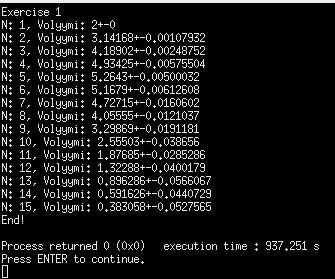
\includegraphics[width=4.3in]{ex1_answer}
    \caption{Ex1 answer.}
    \label{fig:ex1_answer}
\end{figure}

	Result makes sense, since the correct answers are 2, $\pi$, 4*$\pi$/3 ...

\clearpage

\section{Exercise 2}
Answer presented in Figure \ref{fig:ex2_answer}.
\begin{figure}[!hbt]
	\centering
	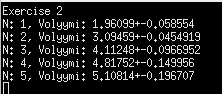
\includegraphics[width=4.3in]{ex2_answer}
	\caption{Ex2 answer.}
	\label{fig:ex2_answer}
\end{figure}

Result in Exercise 1 and Exercise 2 are pretty similar. However the sampling method requires significantly more time, so had to increase binning, which increased the uncertainty.

\clearpage

\section{Exercise 3}
Answer presented in Figure \ref{fig:ex3_answer}.
\begin{figure}[!hbt]
	\centering
	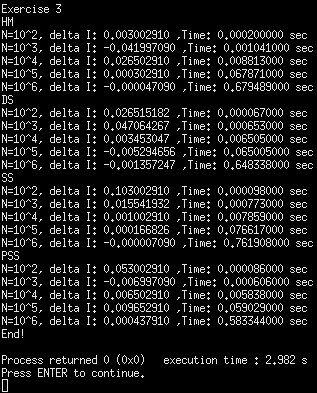
\includegraphics[width=4.3in]{ex3_answer}
	\caption{Ex3 answer.}
	\label{fig:ex3_answer}
\end{figure}

The increase of N looks like increasing the precision of the result.

The strange peak is observed in PSS at N =$10^5$, which suggests that the N is not big enough.

Time increase is as predictable, N multiplication by 10 increases time nearly 10 times.

\clearpage
\section{Exercise 4}
\subsection{a)}
Figure \ref{fig:ex4a_answer}.
\begin{figure}[!hbt]
	\centering
	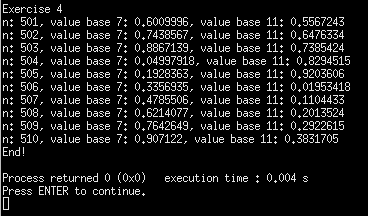
\includegraphics[width=4.3in]{ex4a_answer}
	\caption{Ex4 answer.}
	\label{fig:ex4a_answer}
\end{figure}

\end{document}